\documentclass[tocsection,footlinesection,aspectratio=169,mathserif]{beamer}
\usetheme{cleandigo}
% === LANGUAGES ===
\usepackage[T5]{fontenc}
\usepackage[utf8]{inputenc}
\usepackage[vietnamese]{babel}

% === TYPESET and TEXT LAYOUT ===
% DO NOT USE SETSPACE, it messes with footnote?
% \usepackage{setspace}
% \setstretch{1.3}
% \usepackage{mlmodern}
\usepackage{tgadventor}

% === MATH TYPESETTING ===
\usepackage{amsmath, amsthm, amsfonts, amssymb,
            nicefrac}
% define custom math env
\theoremstyle{definition}
\newtheorem{defn}{Định nghĩa}
\newtheorem{prop}{Mệnh đề}
\newtheorem{thm}{Định lý}
\newtheorem{remark}{Quan sát}
% \newtheorem{example}{Ví dụ}

% spacing of left right
% https://tex.stackexchange.com/questions/2607/spacing-around-left-and-right
\let\originalleft\left
\let\originalright\right
\renewcommand{\left}{\mathopen{}\mathclose\bgroup\originalleft}
\renewcommand{\right}{\aftergroup\egroup\originalright}
% define custom operators
\DeclareMathOperator*{\fbm}{fBM}
\DeclareMathOperator*{\Var}{Var}
\DeclareMathOperator*{\D}{d\!} % Reduce kerning since \operatorname makes some space, \d is already defined
\DeclareMathOperator*{\LayerNorm}{LayerNorm}
\DeclareMathOperator*{\Softmax}{Softmax}
\DeclareMathOperator*{\Attention}{Attention}
\DeclareMathOperator*{\Enc}{enc}
\DeclareMathOperator*{\Dec}{dec}
\newcommand{\Ex}{\operatorname{\mathbb{E}}}
\newcommand{\R}{\mathbb{R}}

% === REFERENCE TYPESETTING ===
% \usepackage[sort,square,numbers]{natbib}
\usepackage{prettyref}
\newrefformat{fig}{Hình \ref{#1}}
\newrefformat{prop}{Mệnh đề \ref{#1}}
\newrefformat{sec}{Mục \ref{#1}}

% Cite author along with the paper
% \let\oldciteauthor\citeauthor
% \renewcommand{\citeauthor}[1]{\oldciteauthor{#1}\textsuperscript{\cite{#1}}}


% === OTHER ELEMENTS ===
\usepackage{url} 
% \usepackage[unicode=true,pdfusetitle,breakbookmarks=true]
%  {hyperref} % hyper links 

\usepackage{subcaption}

% \usepackage[utf8x]{inputenc}

\renewcommand*{\thefootnote}{(\arabic{footnote})}


\usepackage[
    maxcitenames=1,
	maxnames=1,
	% style=ieee,
	sorting=ynt,
    sortcites,
    natbib=true,
    doi=false,
    isbn=false,
    url=false,
    eprint=false,
]{biblatex}
\DefineBibliographyStrings{Vietnamese}{
    in = {trong},
    and = {và},
    andothers = {và các cộng sự}
}
% FOOTNOTE CITATION HACK
% author: ndgnuh
% usage:
% % FOOTNOTE CITATION HACK
% author: ndgnuh
% usage:
% % FOOTNOTE CITATION HACK
% author: ndgnuh
% usage:
% \input{myfootcite} % input this file
% \begin{frame}
%   \cite{MyRef} % first citing
%    ...
%   \cite{MyRef} % second citing of same document
%    \ffcite{MyRef} % This command makes it appears in the footnote
% \end{frame}
\makeatletter

\DeclareCiteCommand{\cite}[\mkbibbrackets]
{%
	%\usebibmacro{cite:init}%
	\usebibmacro{prenote}}
{%
	\usebibmacro{citeindex}%
	%\usebibmacro{cite:comp}%
	\usebibmacro{cite}%
	\ifciteseen
	{}
	{\csnumgdef{cbx@instcount\thefield{entrykey}}{-100}}%
}
{\multicitedelim}
{%
	\usebibmacro{postnote}%
}

\DeclareCiteCommand{\@ffcite}[\cbx@ff]
{%	% precode start
	%precode end
}
{%	% loop code
	\usebibmacro{citeindex}%
	\gdef\cbx@citekey{\thefield{entrykey}}%
	\ifciteseen
	{}% if true, empty
	{%	% if false
		% if cite for the first time
		% the the fakecount to -100
		% this will only run at first cite?
		%				\BibliographyWarning{\cbx@citekey is unseen, ignoring ffcite }%
		\csnumgdef{cbx@instcount\cbx@citekey}{-100}%
	}%
	% end ifciteseen
	% when meet a cite within the same page...
	% compare two item defined by instcount and the fakecount
	\ifsamepage%
	{\value{instcount}} % first value
	{\number\csuse{cbx@instcount\cbx@citekey}}% the value previously set
	{}% do nothing if they are the same
	{% write a footnote if not
		\xappto{\cbx@citehook}{%
			\noexpand\footnotetext[\thefield{labelnumber}]{%
				\fullcite{\thefield{entrykey}}%
			}%
		}%
		%				\gdef\@makefnmark\old@makefnmark
	}%
	\csnumgdef{cbx@instcount\cbx@citekey}{\value{instcount}}%
	%		\usebibmacro{cite:comp}%
	% end loop code
}
{}
{\usebibmacro{postnote}}

\newrobustcmd{\cbx@ff}[1]{%
	\mkbibsuperscript{#1}%
	\cbx@citehook%
	\global\let\cbx@citehook=\empty%
}
\let\cbx@citehook=\empty

\def\citecolor{black}
\newcommand{\ffcite}[1]{%
	\let\old@makefnmark\@makefnmark%
	\let\oldthefootnote\thefootnote%
	\renewcommand{\thefootnote}{[\textcolor{\citecolor}{\arabic{footnote}}]}%
	\renewcommand{\@makefnmark}{\makebox{\normalfont\@thefnmark}}%
	\@ffcite{#1}%
	\renewcommand{\thefootnote}{\oldthefootnote}%
	\renewcommand{\@makefnmark}{\old@makefnmark}%
}

\makeatother
 % input this file
% \begin{frame}
%   \cite{MyRef} % first citing
%    ...
%   \cite{MyRef} % second citing of same document
%    \ffcite{MyRef} % This command makes it appears in the footnote
% \end{frame}
\makeatletter

\DeclareCiteCommand{\cite}[\mkbibbrackets]
{%
	%\usebibmacro{cite:init}%
	\usebibmacro{prenote}}
{%
	\usebibmacro{citeindex}%
	%\usebibmacro{cite:comp}%
	\usebibmacro{cite}%
	\ifciteseen
	{}
	{\csnumgdef{cbx@instcount\thefield{entrykey}}{-100}}%
}
{\multicitedelim}
{%
	\usebibmacro{postnote}%
}

\DeclareCiteCommand{\@ffcite}[\cbx@ff]
{%	% precode start
	%precode end
}
{%	% loop code
	\usebibmacro{citeindex}%
	\gdef\cbx@citekey{\thefield{entrykey}}%
	\ifciteseen
	{}% if true, empty
	{%	% if false
		% if cite for the first time
		% the the fakecount to -100
		% this will only run at first cite?
		%				\BibliographyWarning{\cbx@citekey is unseen, ignoring ffcite }%
		\csnumgdef{cbx@instcount\cbx@citekey}{-100}%
	}%
	% end ifciteseen
	% when meet a cite within the same page...
	% compare two item defined by instcount and the fakecount
	\ifsamepage%
	{\value{instcount}} % first value
	{\number\csuse{cbx@instcount\cbx@citekey}}% the value previously set
	{}% do nothing if they are the same
	{% write a footnote if not
		\xappto{\cbx@citehook}{%
			\noexpand\footnotetext[\thefield{labelnumber}]{%
				\fullcite{\thefield{entrykey}}%
			}%
		}%
		%				\gdef\@makefnmark\old@makefnmark
	}%
	\csnumgdef{cbx@instcount\cbx@citekey}{\value{instcount}}%
	%		\usebibmacro{cite:comp}%
	% end loop code
}
{}
{\usebibmacro{postnote}}

\newrobustcmd{\cbx@ff}[1]{%
	\mkbibsuperscript{#1}%
	\cbx@citehook%
	\global\let\cbx@citehook=\empty%
}
\let\cbx@citehook=\empty

\def\citecolor{black}
\newcommand{\ffcite}[1]{%
	\let\old@makefnmark\@makefnmark%
	\let\oldthefootnote\thefootnote%
	\renewcommand{\thefootnote}{[\textcolor{\citecolor}{\arabic{footnote}}]}%
	\renewcommand{\@makefnmark}{\makebox{\normalfont\@thefnmark}}%
	\@ffcite{#1}%
	\renewcommand{\thefootnote}{\oldthefootnote}%
	\renewcommand{\@makefnmark}{\old@makefnmark}%
}

\makeatother
 % input this file
% \begin{frame}
%   \cite{MyRef} % first citing
%    ...
%   \cite{MyRef} % second citing of same document
%    \ffcite{MyRef} % This command makes it appears in the footnote
% \end{frame}
\makeatletter

\DeclareCiteCommand{\cite}[\mkbibbrackets]
{%
	%\usebibmacro{cite:init}%
	\usebibmacro{prenote}}
{%
	\usebibmacro{citeindex}%
	%\usebibmacro{cite:comp}%
	\usebibmacro{cite}%
	\ifciteseen
	{}
	{\csnumgdef{cbx@instcount\thefield{entrykey}}{-100}}%
}
{\multicitedelim}
{%
	\usebibmacro{postnote}%
}

\DeclareCiteCommand{\@ffcite}[\cbx@ff]
{%	% precode start
	%precode end
}
{%	% loop code
	\usebibmacro{citeindex}%
	\gdef\cbx@citekey{\thefield{entrykey}}%
	\ifciteseen
	{}% if true, empty
	{%	% if false
		% if cite for the first time
		% the the fakecount to -100
		% this will only run at first cite?
		%				\BibliographyWarning{\cbx@citekey is unseen, ignoring ffcite }%
		\csnumgdef{cbx@instcount\cbx@citekey}{-100}%
	}%
	% end ifciteseen
	% when meet a cite within the same page...
	% compare two item defined by instcount and the fakecount
	\ifsamepage%
	{\value{instcount}} % first value
	{\number\csuse{cbx@instcount\cbx@citekey}}% the value previously set
	{}% do nothing if they are the same
	{% write a footnote if not
		\xappto{\cbx@citehook}{%
			\noexpand\footnotetext[\thefield{labelnumber}]{%
				\fullcite{\thefield{entrykey}}%
			}%
		}%
		%				\gdef\@makefnmark\old@makefnmark
	}%
	\csnumgdef{cbx@instcount\cbx@citekey}{\value{instcount}}%
	%		\usebibmacro{cite:comp}%
	% end loop code
}
{}
{\usebibmacro{postnote}}

\newrobustcmd{\cbx@ff}[1]{%
	\mkbibsuperscript{#1}%
	\cbx@citehook%
	\global\let\cbx@citehook=\empty%
}
\let\cbx@citehook=\empty

\def\citecolor{black}
\newcommand{\ffcite}[1]{%
	\let\old@makefnmark\@makefnmark%
	\let\oldthefootnote\thefootnote%
	\renewcommand{\thefootnote}{[\textcolor{\citecolor}{\arabic{footnote}}]}%
	\renewcommand{\@makefnmark}{\makebox{\normalfont\@thefnmark}}%
	\@ffcite{#1}%
	\renewcommand{\thefootnote}{\oldthefootnote}%
	\renewcommand{\@makefnmark}{\old@makefnmark}%
}

\makeatother

\addbibresource{refs.bib}

% \usepackage[numbers,sort]{natbib}
% \usepackage{usebib}
% \usepackage{bibentry}
% \bibinput{refs}
% \nobibliography{refs.bib}
% \newcommand{\citef}[1]{%t
%     \footnote{%
%     \citeauthor{#1}--\textit{\usebibentry{#1}{title}}\cite{#1}
%     }%
% }
% \newcommand{\citefm}[2]{%t
%     \footnotetext[#2]{%
%     \citeauthor{#1}--\textit{\usebibentry{#1}{title}}\cite{#1}
%     }%
% }

\newcommand{\citef}[1]{\cite{#1}\ffcite{#1}}

\newcommand{\Image}[1]{%
	\sbox0{\includegraphics[height=\graphicht]{#1}}%
	\ifdim\wd0 < \textwidth
	\includegraphics[height=\graphicht]{#1}%
	\else
	\includegraphics[width=\textwidth]{#1}%
	\fi%
}

% \newif\iffirsttoc
% \firsttoctrue
% \AtBeginSection[]
% {
% 	\footlinesectiononfalse
%     \begin{frame}{Mục lục}  
%         \iffirsttoc
%             \tableofcontents
%             \global\firsttocfalse
%         \else
%             \tableofcontents[currentsection,
%             % hideothersubsections,
%             subsectionstyle=show/shaded/hide,
%             subsubsectionstyle=show/show/show/hide
%             ]
%         \fi
%     \end{frame} 
% 	\footlinesectionontrue
% }

\usepackage{avant}

% === BEAMER STUFF %%%

% \usepackage{layout}

\begin{document}

\begin{frame}[noframenumbering,plain]{}
	\relax
	\vfill
	{
		\usebeamercolor[fg]{title}{%
			% artistic choice, do not capitalize anything here
			\emph{\large Các mô hình ngẫu nhiên và ứng dụng:}

			{\Large CHUYỂN ĐỘNG BROWN, MÔ HÌNH HỌC SÂU VÀ NHÚNG DỮ LIỆU}
		}

		\medskip

		\hrule
	}

	\vfill

	\textbf{Giảng viên hướng dẫn:} TS.\,Nguyễn Thị Ngọc Anh

	\textbf{Học viên:} Nguyễn Đức Hùng${}\sim{}$20212498M

	\vfill
	Hà Nội, Tháng 03 năm 2023
	\vfill
\end{frame}

% \begin{frame}[Title]
%     \vspace{-5em}
%     \layout
% \end{frame}
\section{Giới thiệu}

\begin{frame}{Giới thiệu}
	\begin{itemize}
		\item Vật lý
		\item Tài chính
		\item ???
	\end{itemize}
\end{frame}

\begin{frame}{Giới thiệu}
	\begin{figure}
		\centering
		
\includegraphics[height=\graphicht]{figures/fbm(p).jpg}
		\caption{%
			Inigo Quilez--$f(p) = \fbm(p+\fbm(p+\fbm(p)))$%
			\footnote[frame]{\url{https://iquilezles.org/articles/warp/}}
		}
		\label{fig:my_label}
	\end{figure}
\end{frame}

\section{Chuyển động Brown}
\begin{frame}[nosection]{Tính chất}
	\begin{prop}\label{prop:nowhere-diff-brown}
		Chuyển động Brown hầu chắc chắn không khả vi
		tại $t>0$\citef{S096:17}.
	\end{prop}
\end{frame}


\begin{frame}{Tính chất}
	\begin{align}
		f\left(x+\Delta x\right)-f\left(x\right)      & =\sum_{k=1}^{\infty}\frac{\left(\Delta x\right)^{k}}{k!}f^{\left(k\right)}\left(x\right) \\
		\Ex\left[\left(\Delta B_{t}\right)^{2}\right] & =\Ex\left[\left(B_{t+\Delta t}-B_{t}\right)^{2}\right]                                   \\
		                                              & =\Var\left[\Delta B_{t}\right]+\Ex\left[\Delta B_{t}\right]=\Delta t.
	\end{align}
\end{frame}

\begin{frame}{Tính chất}
	Giải tích
	\begin{align}
		\D f\left(t,x\right)=\frac{\partial f}{\partial x}\D x+\frac{\partial f}{\partial t}\D t,
	\end{align}
	Giải tích Itô
	\begin{align}
		\D f\left(t,B_{t}\right) & =\frac{\partial f}{\partial x}\D B_{t}+\frac{\partial f}{\partial t}\D t+\frac{1}{2}\cdot\frac{\partial^{2}f}{\partial x^{2}}\left(\D B_{t}\right)^{2} \nonumber \\
		                         & =\left(\frac{\partial f}{\partial t}+\frac{1}{2}\cdot\frac{\partial^{2}f}{\partial x^{2}}\right)\D t+\frac{\partial f}{\partial x}\D B_{t}.\label{eq:ito-diff}
	\end{align}
\end{frame}

	\section{Chuyển động Brown và Transformer}

\subsection{ASDKALSJDALKJ}

\begin{frame}{Một số định nghĩa}
	\begin{defn}[Layer Normalization]
		\begin{equation}
			\LayerNorm\left(x\right)=\frac{x-\Ex\left[x\right]}{\sqrt{\Var\left[x\right]}}\cdot\gamma+\beta,
		\end{equation}
	\end{defn}

	\begin{defn}[Softmax]
		\begin{equation}
			\Softmax\left(x\right)=\left[\frac{\exp\left(x_{j}\right)}{\sum_{i=1}^{d}\exp\left(x_{i}\right)}\right]_{j=\overline{1,d}}
		\end{equation}
	\end{defn}
\end{frame}

\begin{frame}{Một số định nghĩa}
	\begin{defn}[Scale-dot Attention]
		\begin{equation}
			\Attention\left(Q,K,V\right)=\Softmax\left(\frac{QK^{\top}}{\sqrt{d}}\right)\cdot V
		\end{equation}
	\end{defn}
\end{frame}

\begin{frame}{Một số định nghĩa}
	\begin{figure}
		\centering
		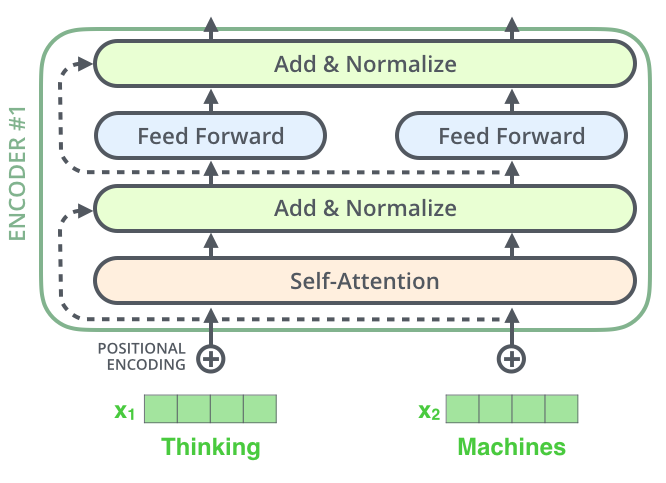
\includegraphics[height=\graphicht]{figures/transformer-layer.png}
		\caption{Một lớp transformer}
	\end{figure}
\end{frame}
\begin{frame}{Quan sát}
	\begin{remark}
		\begin{itemize}
			\item Tính chất chuẩn hoá\citef{LayerNormInTransformer}
			      \begin{equation}
				      \left\lVert \LayerNorm\left(x\right)\right\rVert =\sqrt{d};
			      \end{equation}
			\item Ma trận chuyển\cite{BrownianTransformers}
			      \begin{equation}
				      p_{i,j}=\exp\left(\frac{-\left\lVert v_{i}-v_{j}\right\rVert ^{2}}{2\sqrt{d}}\right);
			      \end{equation}
			\item Thuật toán tối ưu bậc 2\citef{BrownianTransformers}.
		\end{itemize}
	\end{remark}
\end{frame}


\begin{frame}{Quan sát}
	\begin{remark}
		\begin{itemize}
			\item Multi-head?
			\item Kết nối tắt
			      \begin{equation}
				      y = f(x) + x;
			      \end{equation}
			\item Lớp chiếu
			      \begin{equation}
				      y = x\cdot A^{\top} + b.
			      \end{equation}
		\end{itemize}
	\end{remark}
\end{frame}

\section{Chuyển động Brown và $\Delta$VAE}

\begin{frame}[nosection]{VAE}
	\begin{figure}
		\centering
		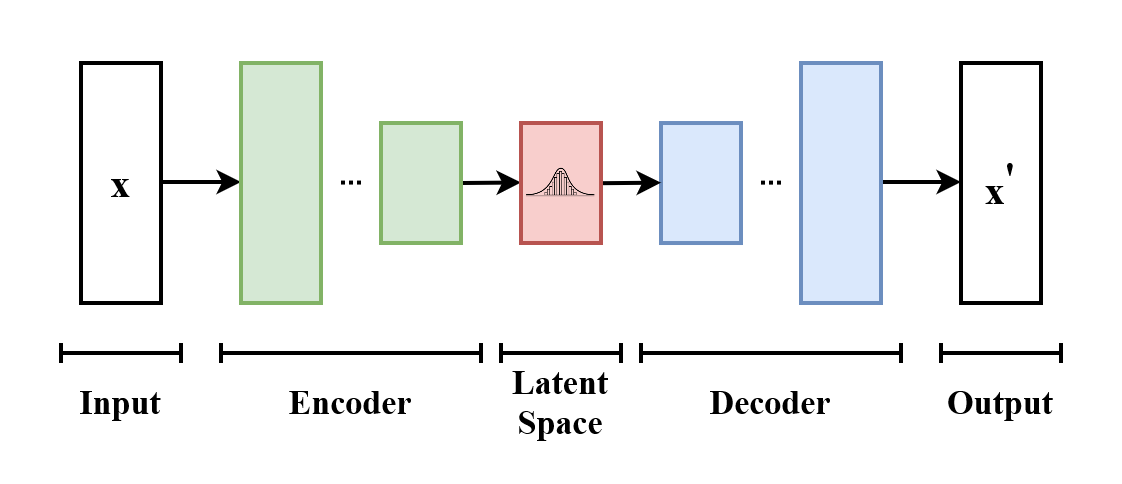
\includegraphics[height=\graphicht]{figures/vae.png}
		\caption{Ý tưởng của VAE}
	\end{figure}
\end{frame}

\begin{frame}{VAE}
	\begin{itemize}
		\item Không gian biến ẩn $Z$;
		\item Phân phối biến ẩn $\mathbb{P}_{Z}$;
		\item Họ phân phối mã hoá $\mathbb{Q}_{Z}$;
		\item Họ phân phối giải mã $\mathbb{P}_{X}$;
		\item Hàm đổi biến $g$.
	\end{itemize}
\end{frame}

\begin{frame}{VAE}
	\begin{defn}[Hàm mục tiêu]
		\begin{equation}
			L\left(x\right)=-\Ex_{z\sim\mathbb{Q}_{Z}^{\boldsymbol{\alpha}\left(x\right)}}\left[\log p_{X}^{\beta\left(z\right)}\left(x\right)\right]+D_{\mathrm{KL}}\left(\mathbb{Q}_{Z}^{\Enc\left(x\right)}\Vert\mathbb{P}_{Z}\right).
		\end{equation}
	\end{defn}
\end{frame}


\begin{frame}{$\Delta$VAE}{Sự phù hợp với dữ liệu}
	\begin{itemize}
		\item Phân phối chuẩn/Gauss?
		\item Không gian $\R^d$?
		\item Không gian con bất kỳ?
	\end{itemize}
\end{frame}

\begin{frame}{$\Delta$VAE}
	\begin{defn}[Xây dựng đổi biến\citef{DiffusionVAE}]
		\begin{align}
			g \colon{}               & \Gamma\times\left(0,\infty\right)\times Z \to Z \\
			g\left(\gamma,t,z\right) & \sim\mathbb{Q}_{Z}^{t,z}
		\end{align}
	\end{defn}
\end{frame}

\begin{frame}{$\Delta$VAE}
	\begin{defn}[{Xây dựng du động ngẫu nhiên}\citef{DiffusionVAE}]
		\begin{align}
			z_{1}  & =P\left(z+\sqrt{\tau}\varepsilon_{1}\right),                                          \\
			z_{2}  & =P\left(P\left(z+\sqrt{\tau}\varepsilon_{1}\right)+\sqrt{\tau} \varepsilon_{2}\right) \\
			\vdots & \nonumber
		\end{align}
	\end{defn}
\end{frame}

\begin{frame}{$\Delta$VAE}
	\begin{figure}
		\centering
		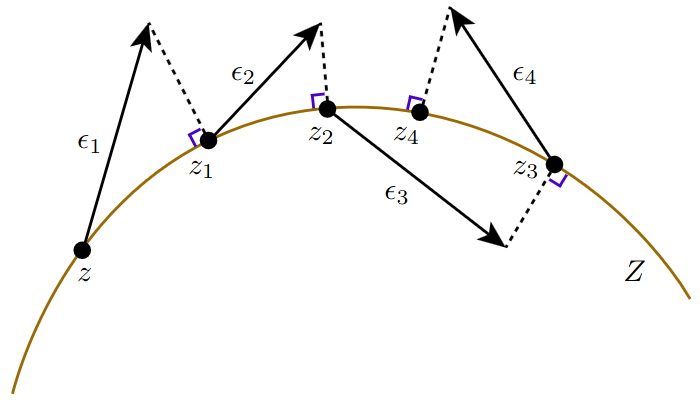
\includegraphics[height=\graphicht]{figures/random-walk-manifold-1d.png}
		\caption{Du động ngẫu nhiên trên một mặt trơn $Z$.\citef{DiffusionVAE}}
		\label{fig:random-walk-manifold}
	\end{figure}
\end{frame}

\begin{frame}{$\Delta$VAE}
	\begin{defn}[Phép đổi biến với chuyển động Brown.\citef{DiffusionVAE}]
		\begin{align}
			g                                                        & \colon\mathcal{E}^{N}\times\left(0,\infty\right)\times Z\to Z,                                                                                            \\
			g\left(\varepsilon_{1},\ldots,\varepsilon_{N},t,z\right) & =P\left(\cdots P\left(P\left(z+\sqrt{\frac{t}{N}}\varepsilon_{1}\right)+\frac{t}{N}\varepsilon_{2}\right)\cdots+\sqrt{\frac{t}{N}}\varepsilon_{N}\right).
		\end{align}
	\end{defn}
\end{frame}

\begin{frame}{$\Delta$VAE}
	\begin{figure}
		\begin{subfigure}{0.49\textwidth}
			\centering
			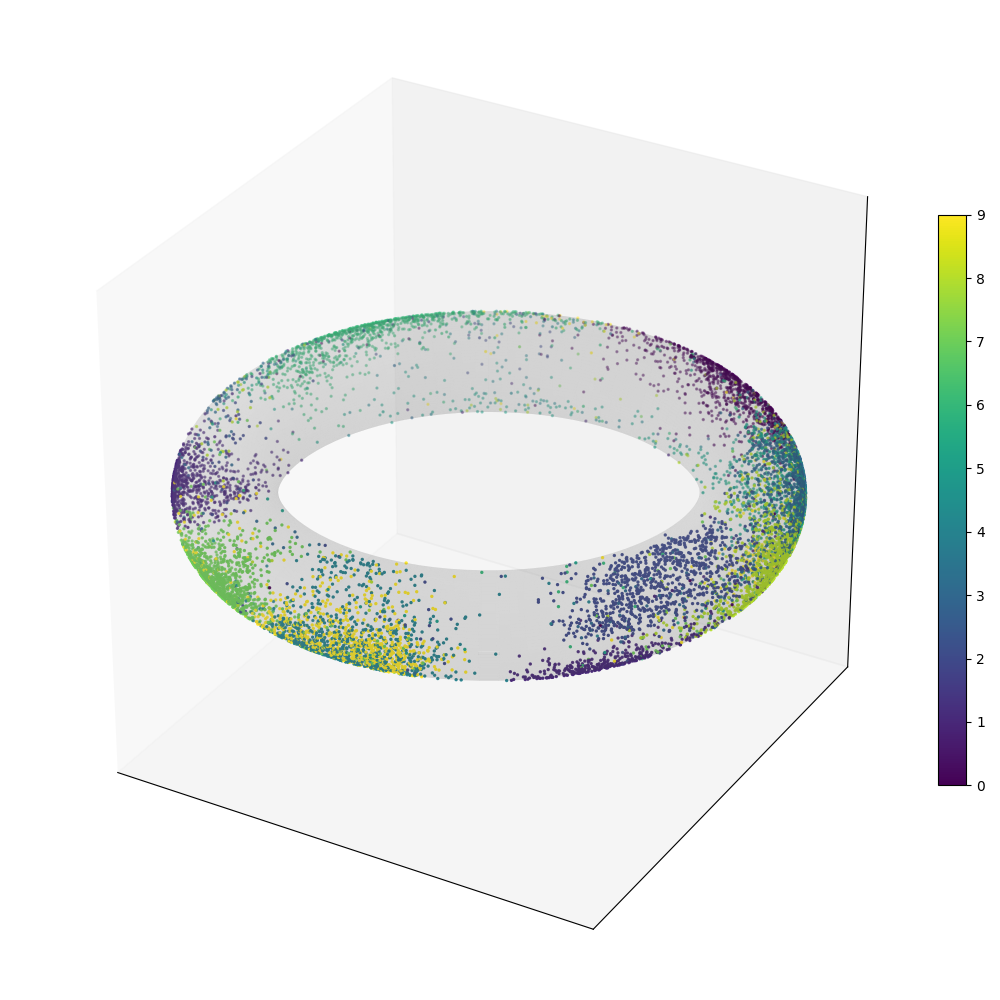
\includegraphics[height=\graphicht]{figures/mnist-latent-torus.png}
			\caption{Mặt hình xuyến}
		\end{subfigure}
		\begin{subfigure}{0.49\textwidth}
			\centering
			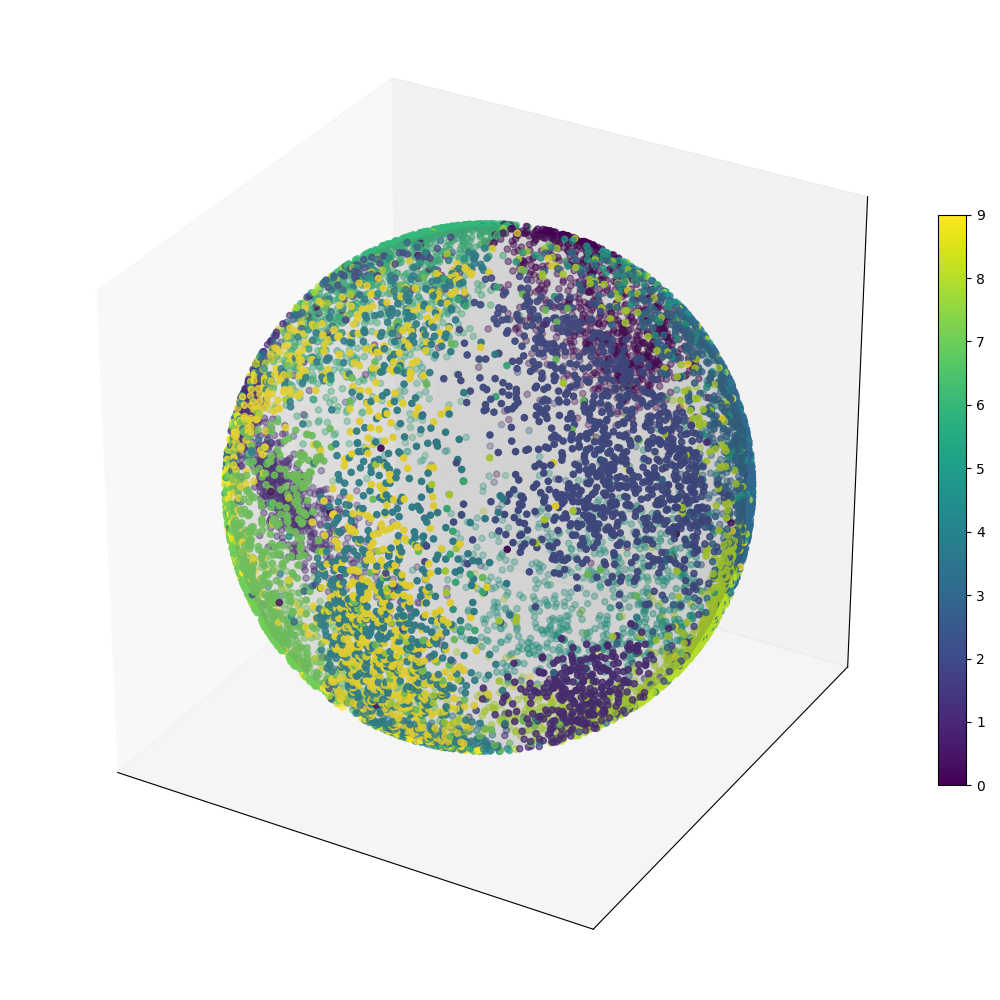
\includegraphics[height=\graphicht]{figures/mnist-latent-sphere_all.png}
			\caption{Cầu đơn vị}
		\end{subfigure}
		\caption{Dữ liệu MNIST nhúng lên các mặt khác nhau}
	\end{figure}
\end{frame}

\section{Kết luận}

\subsection{Kết quả đạt được}
\begin{frame}{Kết luận}
	\begin{itemize}
		\item Dùng chuyển động Brown kết hợp VAE để nhúng dữ liệu;
		\item Transformer $\sim$ kết hợp, biến đổi chuyển động Brown;
		\item Giải thích lỗ hổng trong \citef{BrownianTransformers} với ý tưởng trong \citef{DiffusionVAE};
		\item Nhiều ứng dụng khác.
	\end{itemize}
\end{frame}

\subsection{Cảm ơn}

\begin{frame}{The end}
	Cảm ơn mọi người đã chú ý lắng nghe!
\end{frame}

% \section{Tài liệu tham khảo}
\begin{frame}[fragile,allowframebreaks]{Tài liệu tham khảo}
	% Bài này chứng minh mặt
	\nocite{HSU}
	\printbibliography
	% \bibliographystyle{IEEEtranN}
	% \bibliography{refs.bib}
\end{frame}
\end{document}
